\begin{center}
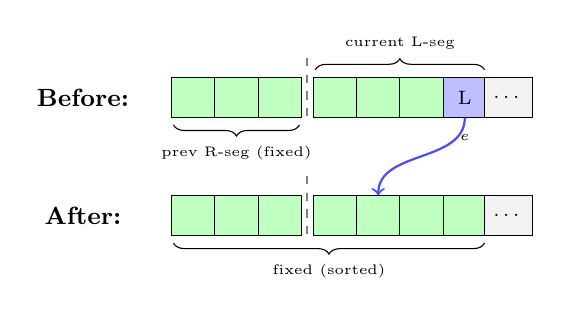
\begin{tikzpicture}[
    cell/.style={minimum width=0.55cm, minimum height=0.5cm, draw, font=\scriptsize},
    fixed/.style={cell, fill=green!25},
    current/.style={cell, fill=blue!25},
    clean/.style={cell, fill=gray!10},
    arrow/.style={->, thick, blue!70},
    boundary/.style={dashed, thick, black!50}
]
% Before state
\node[font=\small\bfseries] at (-1.4, 0) {Before:};
\node[fixed] (f0) at (0, 0) {};
\node[fixed] (f1) at (0.55, 0) {};
\node[fixed] (f2) at (1.1, 0) {};

% Boundary after prev R-seg
\draw[boundary] (1.45, 0.5) -- (1.45, -0.3);

\node[fixed] (f3) at (1.8, 0) {};
\node[fixed] (f4) at (2.35, 0) {};
\node[fixed] (f5) at (2.9, 0) {};
\node[current] (cur) at (3.45, 0) {L};
\node[clean] (c1) at (4.0, 0) {\dots};

% Labels
\draw[decorate, decoration={brace, amplitude=4pt, mirror}] 
    (-0.25, -0.35) -- (1.35, -0.35) node[midway, below=4pt, font=\tiny] {prev R-seg (fixed)};
\draw[decorate, decoration={brace, amplitude=4pt}] 
    (1.55, 0.35) -- (3.7, 0.35) node[midway, above=4pt, font=\tiny] {current L-seg};
\node[font=\tiny, anchor=north] at (3.45, -0.35) {$e$};

% After state
\node[font=\small\bfseries] at (-1.4, -1.5) {After:};
\node[fixed] (af0) at (0, -1.5) {};
\node[fixed] (af1) at (0.55, -1.5) {};
\node[fixed] (af2) at (1.1, -1.5) {};

\draw[boundary] (1.45, -1.0) -- (1.45, -1.8);

\node[fixed] (af3) at (1.8, -1.5) {};
\node[fixed] (acur) at (2.35, -1.5) {};
\node[fixed] (af4) at (2.9, -1.5) {};
\node[fixed] (af5) at (3.45, -1.5) {};
\node[clean] (ac1) at (4.0, -1.5) {\dots};

% Arrow from L in Before to its position in After
\draw[arrow] (cur.south) to[out=-90, in=90] (acur.north);

% Labels after
\draw[decorate, decoration={brace, amplitude=4pt, mirror}] 
    (-0.25, -1.85) -- (3.7, -1.85) node[midway, below=4pt, font=\tiny] {fixed (sorted)};
\end{tikzpicture}
\end{center}